% Options for packages loaded elsewhere
\PassOptionsToPackage{unicode,linktoc=all}{hyperref}
\PassOptionsToPackage{hyphens}{url}
\PassOptionsToPackage{dvipsnames,svgnames,x11names}{xcolor}
%
\documentclass[
  a4paper,
]{article}
\usepackage{amsmath,amssymb}
\usepackage{iftex}
\ifPDFTeX
  \usepackage[T1]{fontenc}
  \usepackage[utf8]{inputenc}
  \usepackage{textcomp} % provide euro and other symbols
\else % if luatex or xetex
  \usepackage{unicode-math} % this also loads fontspec
  \defaultfontfeatures{Scale=MatchLowercase}
  \defaultfontfeatures[\rmfamily]{Ligatures=TeX,Scale=1}
\fi
\usepackage{lmodern}
\ifPDFTeX\else
  % xetex/luatex font selection
\fi
% Use upquote if available, for straight quotes in verbatim environments
\IfFileExists{upquote.sty}{\usepackage{upquote}}{}
\IfFileExists{microtype.sty}{% use microtype if available
  \usepackage[]{microtype}
  \UseMicrotypeSet[protrusion]{basicmath} % disable protrusion for tt fonts
}{}
\makeatletter
\@ifundefined{KOMAClassName}{% if non-KOMA class
  \IfFileExists{parskip.sty}{%
    \usepackage{parskip}
  }{% else
    \setlength{\parindent}{0pt}
    \setlength{\parskip}{6pt plus 2pt minus 1pt}}
}{% if KOMA class
  \KOMAoptions{parskip=half}}
\makeatother
\usepackage{xcolor}
\usepackage[margin=25mm]{geometry}
\usepackage{longtable,booktabs,array}
\usepackage{calc} % for calculating minipage widths
% Correct order of tables after \paragraph or \subparagraph
\usepackage{etoolbox}
\makeatletter
\patchcmd\longtable{\par}{\if@noskipsec\mbox{}\fi\par}{}{}
\makeatother
% Allow footnotes in longtable head/foot
\IfFileExists{footnotehyper.sty}{\usepackage{footnotehyper}}{\usepackage{footnote}}
\makesavenoteenv{longtable}
\usepackage{graphicx}
\makeatletter
\def\maxwidth{\ifdim\Gin@nat@width>\linewidth\linewidth\else\Gin@nat@width\fi}
\def\maxheight{\ifdim\Gin@nat@height>\textheight\textheight\else\Gin@nat@height\fi}
\makeatother
% Scale images if necessary, so that they will not overflow the page
% margins by default, and it is still possible to overwrite the defaults
% using explicit options in \includegraphics[width, height, ...]{}
\setkeys{Gin}{width=\maxwidth,height=\maxheight,keepaspectratio}
% Set default figure placement to htbp
\makeatletter
\def\fps@figure{htbp}
\makeatother
\usepackage{svg}
\setlength{\emergencystretch}{3em} % prevent overfull lines
\providecommand{\tightlist}{%
  \setlength{\itemsep}{0pt}\setlength{\parskip}{0pt}}
\setcounter{secnumdepth}{-\maxdimen} % remove section numbering
\ifLuaTeX
\usepackage[bidi=basic]{babel}
\else
\usepackage[bidi=default]{babel}
\fi
\babelprovide[main,import]{british}
% get rid of language-specific shorthands (see #6817):
\let\LanguageShortHands\languageshorthands
\def\languageshorthands#1{}
% $HOME/.pandoc/defaults/latex-header-includes.tex
% Common header includes for both lualatex and xelatex engines.
%
% Preliminaries
%
% \PassOptionsToPackage{rgb,dvipsnames,svgnames}{xcolor}
% \PassOptionsToPackage{main=british}{babel}
\PassOptionsToPackage{english}{selnolig}
\AtBeginEnvironment{quote}{\small}
\AtBeginEnvironment{quotation}{\small}
\AtBeginEnvironment{longtable}{\centering}
%
% Packages that are useful to include
%
\usepackage{graphicx}
\usepackage{subcaption}
\usepackage[inkscapeversion=1]{svg}
\usepackage[defaultlines=4,all]{nowidow}
\usepackage{etoolbox}
\usepackage{fontsize}
\usepackage{newunicodechar}
\usepackage{pdflscape}
\usepackage{fnpct}
\usepackage{parskip}
  \setlength{\parindent}{0pt}
\usepackage[style=american]{csquotes}
% \usepackage{setspace} Use the <fontname-plus.tex> files for setspace
%
\usepackage{hyperref} % cleveref must come AFTER hyperref
\usepackage[capitalize,noabbrev]{cleveref} % Must come after hyperref
\let\longdivision\relax
\usepackage{longdivision}
% noto-plus.tex
% Font-setting header file for use with Pandoc Markdown
% to generate PDF via LuaLaTeX.
% The main font is Noto Serif.
% Other main fonts are also available in appropriately named file.
\usepackage{fontspec}
\usepackage{setspace}
\setstretch{1.3}
%
\defaultfontfeatures{Ligatures=TeX,Scale=MatchLowercase,Renderer=Node} % at the start always
%
% For English
% See also https://tex.stackexchange.com/questions/574047/lualatex-amsthm-polyglossia-charissil-error
% We use Node as Renderer for the Latin Font and Greek Font and HarfBuzz as renderer ofr Indic fonts.
%
\babelfont{rm}[Script=Latin,Scale=1]{NotoSerif}% Config is at $HOME/texmf/tex/latex/NotoSerif.fontspec
\babelfont{sf}[Script=Latin]{SourceSansPro}% Config is at $HOME/texmf/tex/latex/SourceSansPro.fontspec
\babelfont{tt}[Script=Latin]{FiraMono}% Config is at $HOME/texmf/tex/latex/FiraMono.fontspec
%
% Sanskrit, Tamil, and Greek fonts
%
\babelprovide[import, onchar=ids fonts]{sanskrit}
\babelprovide[import, onchar=ids fonts]{tamil}
\babelprovide[import, onchar=ids fonts]{greek}
%
\babelfont[sanskrit]{rm}[Scale=1.1,Renderer=HarfBuzz,Script=Devanagari]{NotoSerifDevanagari}
\babelfont[sanskrit]{sf}[Scale=1.1,Renderer=HarfBuzz,Script=Devanagari]{NotoSansDevanagari}
\babelfont[tamil]{rm}[Renderer=HarfBuzz,Script=Tamil]{NotoSerifTamil}
\babelfont[tamil]{sf}[Renderer=HarfBuzz,Script=Tamil]{NotoSansTamil}
\babelfont[greek]{rm}[Script=Greek]{GentiumBookPlus}
%
% Math font
%
\usepackage{unicode-math} % seems not to hurt % fallabck
\setmathfont[bold-style=TeX]{STIX Two Math}
\usepackage{amsmath}
\usepackage{esdiff} % for derivative symbols
% \renewcommand{\mathbf}{\symbf}
%
%
% Other fonts
%
\newfontfamily{\emojifont}{Symbola}
%

\usepackage{titling}
\usepackage{fancyhdr}
    \pagestyle{fancy}
    \fancyhead{}
    \fancyfoot{}
    \renewcommand{\headrulewidth}{0.2pt}
    \renewcommand{\footrulewidth}{0.2pt}
    \fancyhead[LO,RE]{\scshape\thetitle}
    \fancyfoot[CO,CE]{\footnotesize Copyright © 2006\textendash\the\year, R (Chandra) Chandrasekhar}
    \fancyfoot[RE,RO]{\thepage}
%
\usepackage{newunicodechar}
\newunicodechar{√}{\textsf{√}}
\ifLuaTeX
  \usepackage{selnolig}  % disable illegal ligatures
\fi
\IfFileExists{bookmark.sty}{\usepackage{bookmark}}{\usepackage{hyperref}}
\IfFileExists{xurl.sty}{\usepackage{xurl}}{} % add URL line breaks if available
\urlstyle{sf}
\hypersetup{
  pdftitle={The Wonder That Is Pi: Part One},
  pdfauthor={R (Chandra) Chandrasekhar},
  pdflang={en-GB},
  colorlinks=true,
  linkcolor={DarkOliveGreen},
  filecolor={Purple},
  citecolor={DarkKhaki},
  urlcolor={Maroon},
  pdfcreator={LaTeX via pandoc}}

\title{The Wonder That Is Pi: Part One}
\author{R (Chandra) Chandrasekhar}
\date{2004-01-14 | 2024-06-29}

\begin{document}
\maketitle

\thispagestyle{empty}


\begin{quote}
This blog began life more than two decades ago, as part of a series of
lectures I delivered to very bright first-year engineering students at
an Australian university.

The number \(\pi\) (pronounced ``pie'') has been recognized from time
immemorial because its physical significance can be grasped easily: it
is the ratio of the circumference of a circle to its diameter. But who
would have thought that such an innocent ratio would exercise such
endless fascination because of the complexities enfolded into it?

Not surprisingly, some students I met recently wanted to know more about
\(\pi\). Accordingly, I have substantially recast and refreshed my
original presentation to better accord with the form and substance of a
blog. The online references have also been updated to keep up with a
rapidly changing Web.

My original intention was to write a single blog on \(\pi\). But because
I did not want it to become another overly long \emph{slog}, I have
decided to divide it into two parts.

If there are any errors or omissions, please
\href{mailto:feedback.swanlotus@gmail.com}{email} me your feedback.
\end{quote}

\subsection{Circumference, diameter, and
π}\label{circumference-diameter-and-ux3c0}

The straight line or
\href{https://mathworld.wolfram.com/Geodesic.html}{geodesic} is the
shortest distance between any two points on a plane, sphere, or other
space. The circle is the
\href{https://en.wikipedia.org/wiki/Locus_(mathematics)}{locus}
traversed by a moving point that is
\href{https://en.wikipedia.org/wiki/Equidistant}{equidistant} from
another fixed point on a two-dimensional plane. It is the most
\href{https://mathworld.wolfram.com/Symmetry.html}{symmetrical} figure
on the plane. The
\href{https://en.wikipedia.org/wiki/Diameter}{diameter} is the name
given both to any straight line passing through the centre of the
circle---intersecting it at two points---as well as to its length. When
we divide the \href{https://en.wikipedia.org/wiki/Perimeter}{perimeter}
of circle, more properly called its
\href{https://en.wikipedia.org/wiki/Circumference}{circumference},
\(C\), by its diameter, \(d\), we get the enigmatic constant \(\pi\),
which has a value between \(3.141\) and \(3.142\):
\begin{equation}\phantomsection\label{eq:pi-Cd}{
\frac{C}{d} = \pi.
}\end{equation} The diameter \(d\) is twice the radius \(r\), and
substituting for \(d\) into \cref{eq:pi-Cd}, we get the well-known
school formula: \begin{equation}\phantomsection\label{eq:two-pi-r}{
C = \pi d = 2\pi r \approx 2\left[\frac{22}{7}\right]r \approx 6.28r.
}\end{equation} Note, however, that \(\pi\) is \emph{not exactly equal}
to \(\frac{22}{7}\). This value is a convenient \emph{rational fraction
approximation} for \(\pi\) that serves well in elementary
contexts.\footnote{See
  \href{https://swanlotus.netlify.app/blogs/a-tale-of-two-measures-degrees-and-radians}{``A
  tale of two measures: degrees and radians''}.}

You might reasonably wonder whether the ratio of the circumference to
the diameter of \emph{any} circle is \emph{always} \(\pi\). The answer
is ``Yes'', because \emph{all circles are similar}. The ratios of
corresponding lengths of similar figures are equal. This idea is also
covered in my blog
\href{https://swanlotus.netlify.app/blogs/a-tale-of-two-measures-degrees-and-radians}{``A
tale of two measures: degrees and radians''}.

The symbol \href{https://en.wikipedia.org/wiki/Pi}{\(\pi\)} is the
lowercase version of the sixteenth letter of the Greek alphabet. For the
history of its use in mathematics, see
\href{https://en.wikipedia.org/wiki/Pi\#Adoption_of_the_symbol_\%CF\%80}{adoption
of the symbol π in Wikipedia}.

\begin{figure}
\centering
\includesvg[width=0.7\textwidth,height=\textheight]{images/C-over-d.svg}
\caption{The ratio of the circumference to the diameter of \emph{any}
circle is \(\pi\).}\label{fig:pi-circle}
\end{figure}

\cref{fig:pi-circle} shows the relationships in \cref{eq:pi-Cd} and
\cref{eq:two-pi-r} pictorially. The circumference of a circle is about
6.28 times its radius. Why this should be so is a secret, a mystery of
Nature.

\subsection{Is π really equal to
22/7?}\label{is-ux3c0-really-equal-to-227}

Is \(\pi\) really equal to \(\frac{22}{7}\), as it has been drummed into
our heads at school? A wonderfully revealing story lies behind this
mysterious relationship, and it is due to the
\href{https://www.collinsdictionary.com/dictionary/english/labours}{labours}
of one man, in the days when calculators could not be dreamed of, and
when neither the decimal system of numbers nor trigonometry were known.
That is the story we look at next.

\subsection{Archimedes of Syracuse}\label{archimedes-of-syracuse}

\href{https://en.wikipedia.org/wiki/Archimedes}{Archimedes of Syracuse}
(Ἀρχιμήδης, 287--212 BCE) was a
\href{https://www.vocabulary.com/dictionary/polymath\#:~:text=Definitions\%20of\%20polymath,of\%20great\%20and\%20varied\%20learning}{polymath}
and genius of the ancient world. He was one of the greatest
mathematicians the world has ever known. By today's standards, he would
be called a mathematician, physicist, engineer, and astronomer,
\href{https://www.ldoceonline.com/dictionary/all-rolled-into-one}{all
rolled into one}. He is perhaps most famous for running out of his
bathtub naked exclaiming
\href{https://www.dictionary.com/browse/eureka}{``Eureka''}---Greek for
``I have found it''---oblivious of those around him. The principle that
he had then discovered---that the upthrust on a body submerged in a
fluid is equal to the weight of fluid displaced---is known as
\href{https://www.britannica.com/science/Archimedes-principle}{Archimedes'
Principle}.

\begin{figure}
\centering
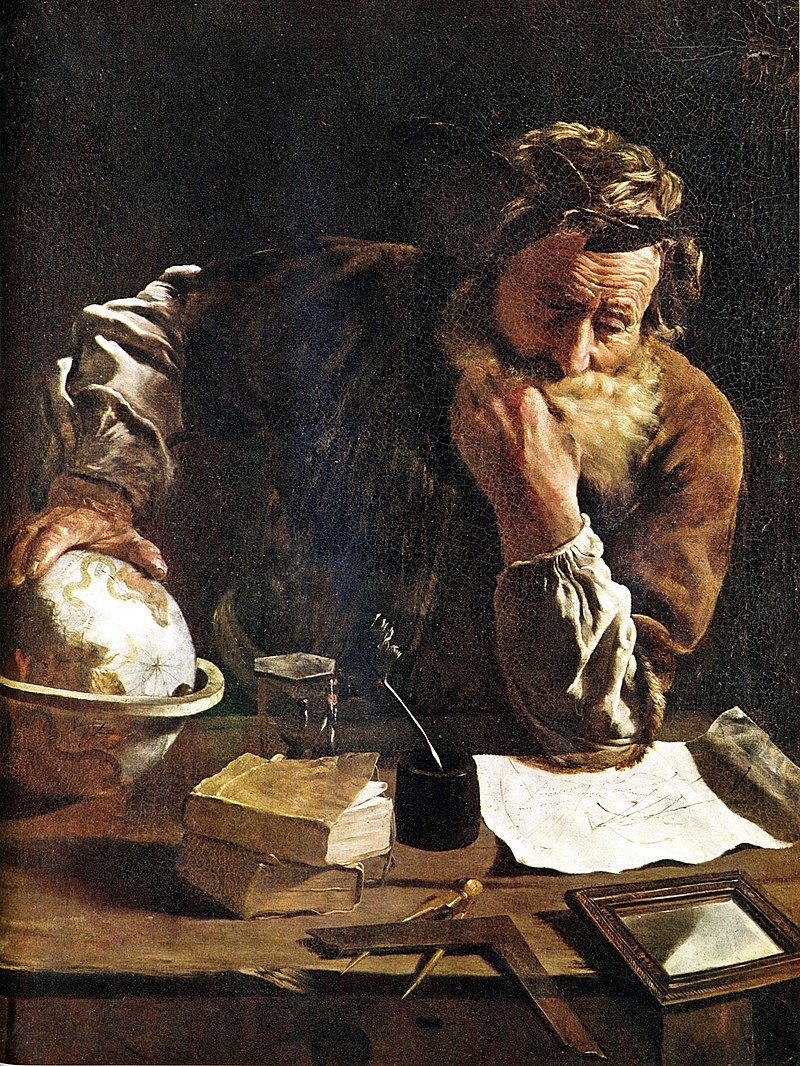
\includegraphics[width=0.7\textwidth,height=\textheight]{images/Domenico-Fetti_Archimedes_1620.jpg}
\caption[Archimedes of Syracuse.]{Archimedes of
Syracuse.\footnotemark{}}\label{fig:archimedes}
\end{figure}
\footnotetext{Domenico Fetti's 1620 painting entitled \emph{Archimedes
  Thoughtful}. Public domain.}

Among the many accomplishments of Archimedes is his method for
estimating \(\pi\), which was the best approximation for almost 1900
years. And it was not based on using a length of string, superimposing
it on a circle, and getting an estimate! What is even more remarkable is
that Archimedes made his discovery without the benefit of either
trigonometry, decimal (positional) notation, or calculators. Instead he
applied the theorem of Pythagoras and extracted square roots laboriously
by hand. His method is also an excellent geometrical illustration of the
idea of a limit, with which he was doubtless familiar. It is known that
Archimedes was familiar with what we now know as integral calculus, and
it is possible that he may have anticipated differential calculus as
well.

He devised an ingenious method for estimating the circumference of a
circle. He used a sophisticated algorithm that allowed him to obtain
successively more accurate values for the circumference of a circle, and
therefore of \(\pi\).

\subsubsection{Principles used by
Archimedes}\label{principles-used-by-archimedes}

The method that Archimedes devised is instructive because it is a
synthesis of several principles by which the greatest human minds have
furthered scientific progress over time. The abstract principles that
Archimedes used to estimate \(\pi\) were these:

\begin{enumerate}
\item
  Start with the known and progress to the unknown;
\item
  Initialize variables;
\item
  Devise a method of increasing the accuracy of the estimate by
  recursion or iteration;
\item
  Stop when the desired accuracy is reached.
\end{enumerate}

These principles constitute what is known as an
\href{https://www.merriam-webster.com/dictionary/algorithm}{algorithm}.
Once such a systematic framework has been put in place, it can be
applied in many research domains to aid rapid scientific progress.

\subsubsection{Of polygons and circles}\label{of-polygons-and-circles}

Archimedes considered a circle with an
\href{https://mathworld.wolfram.com/Inscribed.html}{inscribed} by a
regular polygon with \(n\) sides along with a
\href{https://mathworld.wolfram.com/Circumscribed.html}{circumscribed}
regular polygon with the same \(n\) sides. \cref{fig:two-limits}
illustrates this for the case \(n = 6\), i.e., with a regular
\href{https://www.britannica.com/science/hexagon}{hexagon}.

It is obvious that the \emph{area} of the inscribed hexagon is smaller
than the \emph{area} of the circle, while the \emph{area} of the
circumscribed hexagon exceeds that of the circle. In symbols, with
\(A_i\) representing the area of the inscribed hexagon, \(A\)
representing the area of the circle, and \(A_c\) representing the area
of the circumscribed hexagon, we may say:
\begin{equation}\phantomsection\label{eq:area-inequality}{
A_i < A < A_c.
}\end{equation}

But can we say the same thing about the \emph{perimeters} of these three
objects? This is where the choice of \emph{regular} hexagons makes
matters more tractable. A regular hexagon is composed of six equilateral
triangles, where the length of each side equals the radius. And each
triangle has an area that is the product of half its base multiplied by
its height. But the base equals the radius \(r\) and the height, called
the \href{https://www.mathopenref.com/apothem.html}{apothem} is \(h\).
Therefore the area of one triangle \(A_{\Delta} = \frac{1}{2}rh\). Now
six such triangles sum up to \(\frac{1}{2}6rh\). But \(6r\) is the
perimeter of the hexagon. \emph{Therefore, the area of the regular
hexagon is \(\frac{1}{2}Ph\) where \(P\) is the perimeter of the
hexagon, and \(h\) its apothem}.\footnote{This statement is true of any
  \_regular polygon as well.}

Since the area is proportional to the perimeter, we are justified in
claiming that the magnitudes of the perimeters accord with the
magnitudes of the areas. Therefore, the circumference of the circle,
\(C\), must lie between the perimeter of the inscribed polygon, \(C_i\),
(limit from below) and the perimeter of the circumscribed polygon,
\(C_c\), (limit from above):
\begin{equation}\phantomsection\label{eq:perimeter-inequality}{
C_i < C < C_c.
}\end{equation} Remember this equation because it helps us to estimate
lower and upper bounds for the value of the circumference. Archimedes's
application of the
\href{https://en.wikipedia.org/wiki/Squeeze_theorem}{squeeze theorem}
nineteen centuries before the calculus was invented is illustrated in
\cref{fig:two-limits} and later figures.

\begin{figure}
\centering
\includesvg[width=0.7\textwidth,height=\textheight]{images/two-limits.svg}
\caption{The circumference of the circle in darkolivegreen is bounded
from below by the perimeter of the inscribed hexagon in maroon and
bounded from above by the perimeter of the circumscribed hexagon in
midnightblue. The circumference of the circle must lie between the
perimeters of these two hexagons.}\label{fig:two-limits}
\end{figure}

\subsubsection{Sides of inscribed and circmscribed
polygons}\label{sides-of-inscribed-and-circmscribed-polygons}

\cref{fig:sin-theta-tan-theta} shows the relationship between the sides
of the inscribed and circumscribed polygons.

\begin{figure}
\centering
\includesvg[width=0.7\textwidth,height=\textheight]{images/sin-theta-tan-theta.svg}
\caption{The relationship between the lengths of the incsribed and
circumscribed regular polygons used in the algrithm of Archimedes to
estimate \(\pi\).}\label{fig:sin-theta-tan-theta}
\end{figure}

\subsubsection{The thirty, sixty, ninety right
triangle}\label{the-thirty-sixty-ninety-right-triangle}

Archimedes applied the same principle ``of starting from the known'' to
initiate his algorithm using a regular hexagon, which is a mosaic of six
juxtaposed equilateral triangles. We know from symmetry that each angle
of an equilateral triangle is \(60°\). When an equilateral triangle is
bisected, we get two right angled triangles with angles of thirty and
sixty degrees, as shown in \cref{fig:thirty-sixty}.

\begin{figure}
\centering
\includesvg[width=0.4\textwidth,height=\textheight]{images/thirty-sixty.svg}
\caption{This right-angled, obtained by bisecting an equilateral
triangle, must be familiar to all school students. These
lengths---obtainable from symmetry and the theorem of
Pythagoras---allowed Archimedes to start off his process for estimating
\(\pi\).}\label{fig:thirty-sixty}
\end{figure}

The inscribed hexagon, within a circle of radius one unit, also has a
side of one unit. Thus, the hypotenuse of the circle \(OAP\) in
\cref{fig:thirty-sixty} has unit length. Moreover, the base \(OP\),
resulting from a bisected side, has a length of half a unit. By applying
the theorem of Pythagoras, the third side, \(AP\) is \[
\sqrt{1^2 - \left(\frac{1}{2}\right)^2} = \frac{\sqrt{3}}{2}.
\]

\subsubsection{Extracting square roots by
hand}\label{extracting-square-roots-by-hand}

Archimedes must have known how to extract square roots by hand, and the
value of \(\sqrt{3}\) was one whose value he knew as a rational
fraction. Perhaps, he used one of the methods described in my blog
\href{https://swanlotus.netlify.app/blogs/how-are-numbers-built}{``How
Are Numbers Built?''}. With remarkable accuracy, he stated that
\begin{equation}\phantomsection\label{eq:sqrt3}{\sqrt{3} \approx \frac{265}{153} \approx 1.732.
}\end{equation}

\subsubsection{Recursion and Iteration}\label{recursion-and-iteration}

Archimedes started with regular hexagons and successively doubled the
number of sides, until he had the circle sandwiched between two 96-gons.
Successively doubling or halving is a fast-converging technique used in
numerical estimation when mathematics is applied to solving a variety of
problems. That Archimedes was aware of it shows how far ahead of his
time his thinking was.

He repeatedly calculated rational approximations to \(\pi\) until he was
satisfied with the accuracy. The principle of the method is clearly seen
in \cref{fig:six-gon} to \cref{fig:ninety-six-gon}.

\begin{figure}
\centering
\includesvg[width=0.7\textwidth,height=\textheight]{images/six-gon.svg}
\caption{The estimate for \(\pi\) lies between
\(C_i = 3.0000 < \pi < C_c = 3.4641\).}\label{fig:six-gon}
\end{figure}

\begin{figure}
\centering
\includesvg[width=0.7\textwidth,height=\textheight]{images/twelve-gon.svg}
\caption{The estimate for \(\pi\) lies between
\(C_i = 3.1058 < \pi < C_c = 3.2153\).}\label{fig:twelve-gon}
\end{figure}

\begin{figure}
\centering
\includesvg[width=0.7\textwidth,height=\textheight]{images/twenty-four-gon.svg}
\caption{The estimate for \(\pi\) lies between
\(C_i = 3.1326 < \pi < C_c = 3.1596\).}\label{fig:twenty-four-gon}
\end{figure}

\begin{figure}
\centering
\includesvg[width=0.7\textwidth,height=\textheight]{images/forty-eight-gon.svg}
\caption{The estimate for \(\pi\) lies between
\(C_i = 3.1393 < \pi < C_c = 3.1460\).}\label{fig:forty-eight-gon}
\end{figure}

\begin{figure}
\centering
\includesvg[width=0.7\textwidth,height=\textheight]{images/ninety-six-gon.svg}
\caption{The estimate for \(\pi\) lies between
\(C_i = 3.1410 < \pi < C_c = 3.1427\). Notice in this sequence of images
how the circumference of the circle approaches the perimeter of the
inscribed and circumscribed heaxgons to the point of being
indistinguishable from them.\emph{The final estimate of Archimedes was
\(\frac{223}{71} < \pi < \frac{22}{7}\).}}\label{fig:ninety-six-gon}
\end{figure}

\subsection{Lessons from this
derivation}\label{lessons-from-this-derivation}

Iteration, recursion, bisection, squeeze, etc.

\subsection{A closer look at π}\label{a-closer-look-at-ux3c0}

Pi is both an
\href{https://en.wikipedia.org/wiki/Irrational_number}{irrational} and a
\href{https://en.wikipedia.org/wiki/Transcendental_number}{transcendental}
number. Let us see what each of these
\href{https://www.merriam-webster.com/dictionary/appellation}{appelations}
mean.

Recurring decimals.

\subsection{To explore further}\label{to-explore-further}

A well-written, accessible article on how Archimedes estimated that
\(\pi\) is approximately \(\frac{22}{7}\) is available online:
\href{https://publications.azimpremjiuniversity.edu.in/3356/1/02-DaminiAndAbhishek_PiIs22By7_Final.pdf}{``How
Archimedes showed that pi is approximately 22 by 7''}. I urge you to
read it.\footnote{This article is all the more remarkable because its
  first author is a Grade 8 student: proof that deep mathematics is not
  beyond the school student.} You will then appreciate for yourselves
how arduous the process must have been in an age without the benefit of:
\#. Trigonometry; he used the theorem of pythagors instead; \#. Algebra;
he used geometry and the ratios of the lengths of well-known triangles;
\#. Decimal numbers for division; he used fractions instead; square
roots by hand; similar and congruent figures; bisection theorems;
exhaustion methods

In the series \cref{fig:six} to \cref{fig:forty-eight} below, which
illustrate the approach Archimedes took to estimate \(\pi\), we see very
clearly that the perimeter of the \emph{inscribed polygon} \(c_n\) and
the perimeter of the \emph{circumscribed polygon} \(C_n\) represent
respectively the \emph{lower bound} and \emph{upper bound} of the
estimated value of \(\pi\). As the number of sides, \(n\), of the
polygon increases, the estimates become increasingly accurate.

https://publications.azimpremjiuniversity.edu.in/3356/1/02-DaminiAndAbhishek\_PiIs22By7\_Final.pdf

https://azimpremjiuniversity.edu.in/at-right-angles

\subsubsection{How did Archimedes arrive at π =
22/7?}\label{how-did-archimedes-arrive-at-ux3c0-227}

22/7 = 3.142857 142857 142857 (recurring decimal)

\subsection{Formulae involving π}\label{formulae-involving-ux3c0}

\subsection{Quest for the endless digits of
π}\label{quest-for-the-endless-digits-of-ux3c0}

\subsection{Buffon's Needle}\label{buffons-needle}

\subsection{π Trivia}\label{ux3c0-trivia}

\subsection{Web links}\label{web-links}

https://www.pbs.org/wgbh/nova/physics/approximating-pi.html

https://demonstrations.wolfram.com/ArchimedesApproximationOfPi/ John
Tucker ``Archimedes' Approximation of Pi''
http://demonstrations.wolfram.com/ArchimedesApproximationOfPi/ Wolfram
Demonstrations Project Published: March 5 2009

https://math.stackexchange.com/questions/4851929/archimedes-method-to-estimate-pi

http://arxiv.org/pdf/2008.07995

https://mathsciencehistory.com/2019/10/01/archimedes-and-his-pi-the-great-numerical-hope/

https://carmamaths.org/resources/jon/pi-culture.pdf

https://nonagon.org/ExLibris/archimedes-pi

https://www.exploratorium.edu/pi/history-of-pi

https://en.wikipedia.org/wiki/Approximations\_of\_\%CF\%80

\subsection{Book References}\label{book-references}

\subsection{Web resources}\label{web-resources}

\subsection{Teaser: are of circle half radius multiplied by
circumference.
How?}\label{teaser-are-of-circle-half-radius-multiplied-by-circumference.-how}

\subsection{Appendix: Circumscribed and inscribed polygons of
circle}\label{appendix-circumscribed-and-inscribed-polygons-of-circle}

Archimedes devised his ingenious \emph{squeeze} method for computing the
upper and lower bounds of the perimeter of a circle by computing instead
the perimeters of the polygons that inscribe and circumscribe the
circle. The approximations become more accurate as the number of sides,
\(n\), of the polygon is increased.
\href{https://www.youtube.com/watch?v=_qdnyw5Eb_Y}{This YouTube
presentation} might help you understand the algorithm of Archimedes
better, but remember that he did not have trigonometry to aid hm.

\subsection{Feedback}\label{feedback}

Please \href{mailto:feedback.swanlotus@gmail.com}{email me} your
comments and corrections.

\noindent A PDF version of this article is
\href{./the-wonder-that-is-pi.pdf}{available for download here}:

\begin{small}

\begin{sffamily}

\url{https://swanlotus.netlify.app/blogs/the-wonder-that-is-pi.pdf}

\end{sffamily}

\end{small}



\end{document}
